\documentclass[11pt]{article}

% ============================================================
% PACKAGES
% ============================================================

\usepackage[a4paper,margin=1in]{geometry}
\usepackage{amsmath}
\usepackage{amssymb}
\usepackage{booktabs}
\usepackage{graphicx}
\usepackage{float}
\usepackage{natbib}
\usepackage{xcolor}
\usepackage{microtype}
\usepackage{enumitem}
\usepackage[hidelinks]{hyperref}

\graphicspath{{../results/figures/}}

\setlength{\parindent}{0pt}
\setlength{\parskip}{0.55em}

% ============================================================
% DOCUMENT
% ============================================================

\title{
When Historical Predictions Become Stale:\\
Robust Expert Combination under Temporal Behavioral Shift
}

\author{
\textbf{Ng Jing Yi, Clara}\\
Independent Research Study in Machine Learning and Online Algorithms\\
\texttt{ngjingyiclara@gmail.com}\\
\href{https://github.com/ngclara07/robust_prediction_learning}
{github.com/ngclara07/robust\_prediction\_learning}
}

\date{\today}

\begin{document}

\maketitle

% ============================================================
% ABSTRACT
% ============================================================

\begin{abstract}

Machine-learning systems deployed on sequential behavioral data
frequently rely on predictors trained from historical observations.
Such predictors may become unreliable when user behavior changes over
time. This study investigates when historical predictions should be
trusted and whether behavioral distribution shift can provide a useful
signal for robust prediction combination.

We study this problem using the Last.fm-1K music-listening dataset.
After preprocessing, the experimental corpus contains approximately
18.5 million timestamped interactions from 966 users and 41,045
artists. A Bayesian Personalized Ranking (BPR) model is trained on
historical implicit feedback and evaluated under chronological splits.
Behavioral shift is quantified using Jensen--Shannon divergence between
historical artist distributions and equal-interaction future windows.

Across 6,642 validation windows from 595 sufficiently active users,
behavioral shift is negatively associated with frozen historical-model
quality: the pooled Spearman correlation between shift and
EventMass@20 is $-0.359$, the median within-user correlation is
$-0.252$, and 70.1\% of users with valid correlations exhibit a
negative relationship. This qualitative result remains stable for
window sizes of 125, 250, and 500 interactions.

We subsequently compare five sequential strategies: historical
prediction only, online adaptation only, a static mixture, Hedge, and a
shift-aware adaptive trust mechanism. On the held-out test stream,
online adaptation achieves the highest expected EventMass@20
($0.358$), followed by Hedge ($0.319$). The proposed shift-aware
mechanism reaches $0.240$, outperforming exclusive reliance on the
historical predictor ($0.063$) but not generic loss-adaptive
aggregation.

The results indicate that behavioral shift is informative about
historical-predictor degradation, while also showing that an explicit
shift signal alone is insufficient to outperform rapid online
adaptation in the studied setting. The negative result identifies an
important distinction between detecting distribution shift and
optimally responding to it.

\end{abstract}

% ============================================================
% 1. INTRODUCTION
% ============================================================

\section{Introduction}

Machine-learning models are commonly trained on historical data and
then deployed under the implicit assumption that future observations
remain sufficiently similar to their training distribution. In
sequential applications, this assumption is often violated. User
preferences evolve, new items appear, and environmental conditions
change. Consequently, a predictor that was previously accurate can
become stale.

This problem is related to concept drift and non-stationary learning,
where the statistical properties relevant to prediction change over
time \citep{gama2014survey}. It is also related to the emerging
literature on \emph{algorithms with predictions}, which studies how
classical algorithms can benefit from machine-learned advice while
remaining robust when that advice is inaccurate
\citep{lykouris2018competitive,mitzenmacher2022algorithms}.

Recommender systems provide a useful real-world testbed for this
problem. Historical listening behavior can be used to estimate
personalized preferences, but musical interests can change
substantially over time. Furthermore, recommendation data are typically
implicit, sparse, long-tailed, and temporally structured
\citep{adomavicius2005toward,celma2010music}.

This study asks the following central research question:

\begin{quote}
\textbf{Can behavioral distribution shift be used to determine when a
sequential learning algorithm should reduce its trust in a historical
machine-learning predictor?}
\end{quote}

We first establish whether measurable behavioral shift is associated
with deterioration in a historical recommender. We then formulate the
problem as online combination of two experts:

\begin{enumerate}[label=(\roman*)]
    \item a frozen historical BPR predictor; and
    \item a lightweight online predictor that adapts to recent
    interactions.
\end{enumerate}

Several combination strategies are compared, including a fixed convex
mixture, the Hedge algorithm, and a shift-aware adaptive trust
mechanism.

The principal contributions of this independent study are:

\begin{enumerate}
    \item a reproducible chronological evaluation pipeline for
    studying historical-predictor degradation on approximately
    18.5 million Last.fm listening events;

    \item an empirical analysis showing that larger Jensen--Shannon
    divergence from historical listening distributions is consistently
    associated with lower historical-predictor quality;

    \item a robustness analysis demonstrating that this association
    remains qualitatively stable across multiple temporal window sizes;

    \item an online expert-combination formulation for comparing
    prediction-only, adaptation-only, static, loss-adaptive, and
    distribution-shift-aware strategies; and

    \item a negative but informative result: the proposed shift-aware
    trust rule improves substantially over exclusive reliance on stale
    historical predictions, but does not outperform either pure online
    adaptation or Hedge under the present formulation.
\end{enumerate}

This last result is particularly important. Detecting that a
distribution has changed is not equivalent to knowing how much
historical information should be retained. The experiments therefore
suggest that reliable prediction augmentation requires both a
meaningful shift signal and an effective adaptation mechanism.

% ============================================================
% 2. RELATED WORK
% ============================================================

\section{Related Work}

\subsection{Implicit-Feedback Recommendation}

Recommender systems estimate user preferences from observed interaction
data \citep{adomavicius2005toward}. Music recommendation is
particularly challenging because listening behavior is highly
long-tailed and repeated consumption is common
\citep{celma2010music}.

Bayesian Personalized Ranking (BPR) was introduced for learning
personalized rankings from implicit feedback
\citep{rendle2009bpr}. Given a user $u$, an observed item $i$, and an
unobserved item $j$, BPR learns parameters that increase the pairwise
preference score
%
\begin{equation}
    \hat{x}_{uij}
    =
    \hat{x}_{ui}
    -
    \hat{x}_{uj}.
\end{equation}
%
For matrix factorization, user and item representations are optimized
using a pairwise logistic objective.

In this study, BPR is not intended as a state-of-the-art recommender.
Instead, it serves as a learned historical predictor whose reliability
can be studied as behavior changes.

\subsection{Temporal Distribution Shift}

Concept drift describes settings in which relationships relevant to
prediction evolve over time \citep{gama2014survey}. Such changes can
invalidate models trained under earlier distributions and motivate
continuous adaptation.

We quantify behavioral change using Jensen--Shannon divergence
\citep{lin1991divergence}. For two discrete distributions $P$ and $Q$,
let
%
\begin{equation}
    M = \frac{1}{2}(P+Q).
\end{equation}
%
The Jensen--Shannon divergence is
%
\begin{equation}
    \operatorname{JS}(P,Q)
    =
    \frac{1}{2}
    D_{\mathrm{KL}}(P\|M)
    +
    \frac{1}{2}
    D_{\mathrm{KL}}(Q\|M).
\end{equation}
%
Using logarithms base two yields a bounded quantity in $[0,1]$.

\subsection{Online Learning and Algorithms with Predictions}

Online learning studies sequential decision-making when outcomes are
revealed after predictions are made. The Hedge algorithm uses
multiplicative weight updates to allocate increasing weight to experts
with lower observed loss \citep{freund1997decision}.

For expert $i$ with loss $\ell_{i,t}$, Hedge performs an update of the
form
%
\begin{equation}
    w_{i,t+1}
    \propto
    w_{i,t}
    \exp(-\eta \ell_{i,t}),
\end{equation}
%
where $\eta>0$ is a learning-rate parameter.

More recent work on algorithms with predictions investigates how
machine-learned advice can improve algorithmic decisions without
sacrificing robustness when predictions fail
\citep{lykouris2018competitive,mitzenmacher2022algorithms}.
The present study adopts this perspective: historical BPR scores are
treated as learned advice rather than as an unquestioned source of
truth.

% ============================================================
% 3. DATA
% ============================================================

\section{Dataset and Preprocessing}

\subsection{Last.fm-1K}

Experiments use the Last.fm-1K music recommendation dataset collected
by \citet{celma2010lastfm} from the Last.fm service
\citep{lastfm}. The original data contain timestamped listening events
with user, artist, and track information.

The study operates at the artist level. Artist names are normalized and
used as operational item identifiers because MusicBrainz identifiers
are missing for a substantial portion of the original records.

Users with fewer than 100 retained interactions and artists with fewer
than 20 retained interactions are filtered. After preprocessing, the
dataset contains the statistics shown in Table~\ref{tab:dataset}.

\begin{table}[H]
\centering
\caption{Preprocessed dataset statistics.}
\label{tab:dataset}
\begin{tabular}{lr}
\toprule
Statistic & Value \\
\midrule
Raw listening events & 19,098,853 \\
Processed listening events & 18,521,447 \\
Users & 966 \\
Artists & 41,045 \\
Earliest timestamp & 14 February 2005 \\
Latest timestamp & 29 September 2013 \\
Training interactions & 12,964,572 \\
Validation interactions & 1,852,070 \\
Test interactions & 3,704,805 \\
\bottomrule
\end{tabular}
\end{table}

A per-user chronological split is used:

\[
70\% \text{ training},
\qquad
10\% \text{ validation},
\qquad
20\% \text{ test}.
\]

No random interaction shuffling is performed. For each user, all
training events precede validation events, which in turn precede test
events.

The preprocessing pipeline automatically verifies this temporal
ordering to prevent future-to-past leakage.

\subsection{Exploratory Characteristics}

The artist-frequency distribution is strongly long-tailed: a small
number of artists account for very large interaction volumes while
many artists have relatively few interactions. User activity is also
highly heterogeneous.

The global interaction timeline contains an abrupt reduction in
observed events after approximately 2009. This pattern is treated as a
dataset-coverage artifact rather than direct evidence of behavioral
change. Consequently, our primary drift analysis does not use fixed
calendar months. Instead, equal-interaction windows are constructed
separately for each user.

% ============================================================
% 4. HISTORICAL PREDICTOR
% ============================================================

\section{Historical Recommendation Model}

\subsection{BPR Training}

Repeated listening events are collapsed into unique user--artist
positive pairs when fitting BPR. The historical model therefore learns
implicit preference from whether a user has interacted with an artist,
rather than allowing repeated plays alone to dominate optimization.

The selected BPR configuration is:

\begin{table}[H]
\centering
\caption{BPR hyperparameters selected using validation data.}
\label{tab:bprparams}
\begin{tabular}{lr}
\toprule
Parameter & Value \\
\midrule
Latent factors & 64 \\
Learning rate & 0.05 \\
Regularization & 0.005 \\
Epochs & 5 \\
Batch size & 8,192 \\
Maximum sampled pairs per epoch & 500,000 \\
\bottomrule
\end{tabular}
\end{table}

\subsection{Chronological Baseline}

Table~\ref{tab:baseline} compares BPR against a global popularity
baseline on the chronological test split.

\begin{table}[H]
\centering
\caption{Chronological recommendation baseline performance.}
\label{tab:baseline}
\begin{tabular}{lrrrr}
\toprule
Model
& Precision@20
& Recall@20
& NDCG@20
& MRR@20 \\
\midrule
Popularity
& 0.0886
& \textbf{0.0242}
& \textbf{0.0976}
& \textbf{0.2462} \\
BPR
& \textbf{0.0894}
& 0.0232
& 0.0937
& 0.2131 \\
\bottomrule
\end{tabular}
\end{table}

BPR is therefore useful as a personalized learned predictor but is not
uniformly superior to popularity on the later test period. This
observation motivates studying how predictive usefulness changes over
time rather than assuming that historical personalization remains
reliable indefinitely.

% ============================================================
% 5. TEMPORAL SHIFT ANALYSIS
% ============================================================

\section{Temporal Behavioral Shift}

\subsection{Equal-Interaction Windows}

For each user $u$, the validation interaction stream is divided
chronologically into windows containing a fixed number of listening
events. The primary analysis uses 250 interactions per window and
requires at least three complete windows per user.

Let
%
\begin{equation}
    P_u^{H}
\end{equation}
%
denote the normalized historical artist distribution for user $u$, and
let
%
\begin{equation}
    P_{u,t}
\end{equation}
%
denote the artist distribution in future window $t$.

Behavioral shift is defined as
%
\begin{equation}
    s_{u,t}
    =
    \operatorname{JS}
    \left(
        P_u^{H},
        P_{u,t}
    \right).
\end{equation}

\subsection{EventMass@K}

Repeated listening is meaningful in music consumption. We therefore
supplement binary ranking metrics with EventMass@K.

For recommendation set $R_{u,t}^{K}$ and event counts
$n_{u,t}(i)$,
%
\begin{equation}
    \operatorname{EventMass@K}_{u,t}
    =
    \frac{
        \sum_{i\in R_{u,t}^{K}}
        n_{u,t}(i)
    }{
        \sum_j n_{u,t}(j)
    }.
\end{equation}

This measures the fraction of actual listening activity covered by the
recommended top-$K$ artists.

\subsection{Shift and Predictor Quality}

At the primary window size of 250 interactions, 595 users provide at
least three complete validation windows, producing 6,642 windows.

The mean Jensen--Shannon divergence from historical behavior is
$0.642$, with median $0.663$. The mean fraction of events involving
artists globally unavailable to the historical model is only 1.03\%,
while approximately 14.1\% of future events involve artists not
previously observed for the corresponding user.

The pooled Spearman correlation between behavioral shift and historical
BPR EventMass@20 is
%
\begin{equation}
    \rho = -0.359.
\end{equation}
%
For BPR NDCG@20, the pooled Spearman correlation is
%
\begin{equation}
    \rho = -0.484.
\end{equation}

Because windows belonging to the same user are not statistically
independent, pooled significance tests are not treated as the main
inferential evidence. Instead, we compute a separate Spearman
correlation within each user. Among 562 users with valid within-user
correlations, the median is
%
\begin{equation}
    \operatorname{median}(\rho_u)
    =
    -0.252,
\end{equation}
%
and 70.1\% have $\rho_u<0$.

Figure~\ref{fig:shiftquality} illustrates the relationship.

\begin{figure}[H]
    \centering
    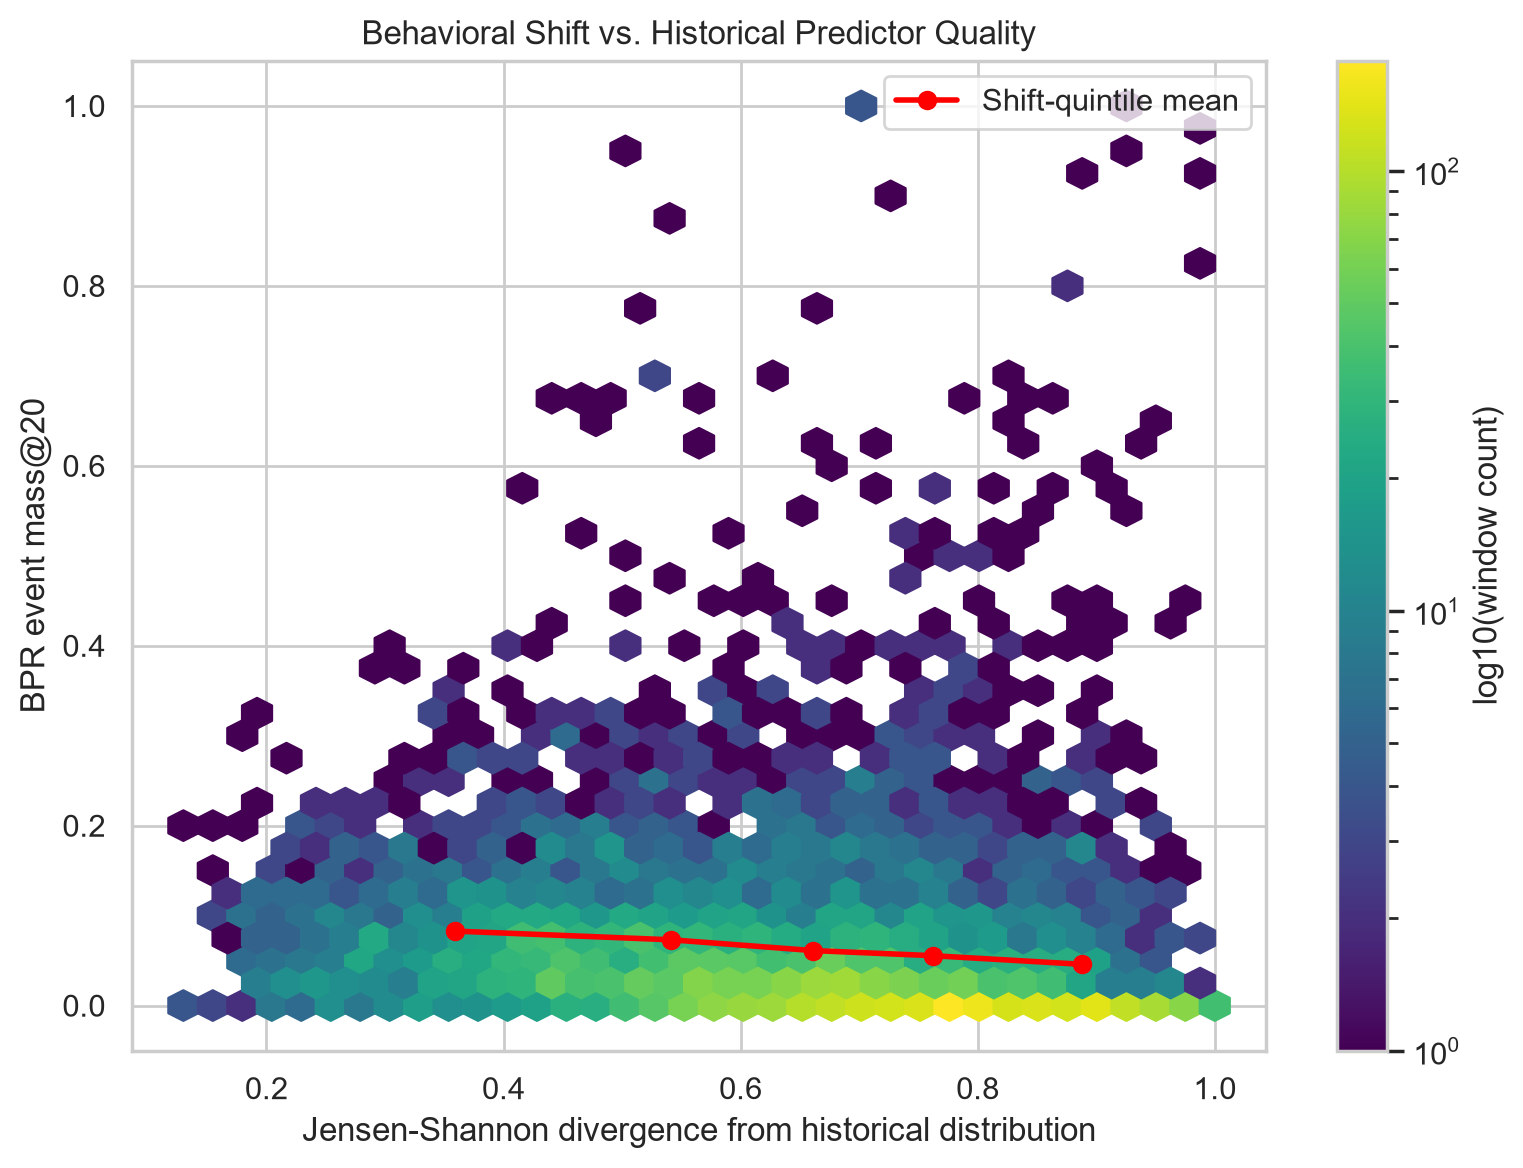
\includegraphics[
        width=0.88\linewidth
    ]{shift_vs_prediction_quality.png}
    \caption{
    Behavioral shift versus frozen historical BPR quality.
    Hexagonal density cells summarize validation windows; the red line
    reports mean EventMass@20 across shift quintiles. Larger divergence
    is associated with lower historical-predictor coverage.
    }
    \label{fig:shiftquality}
\end{figure}

The distribution of within-user correlations is shown in
Figure~\ref{fig:usercorrelation}.

\begin{figure}[H]
    \centering
    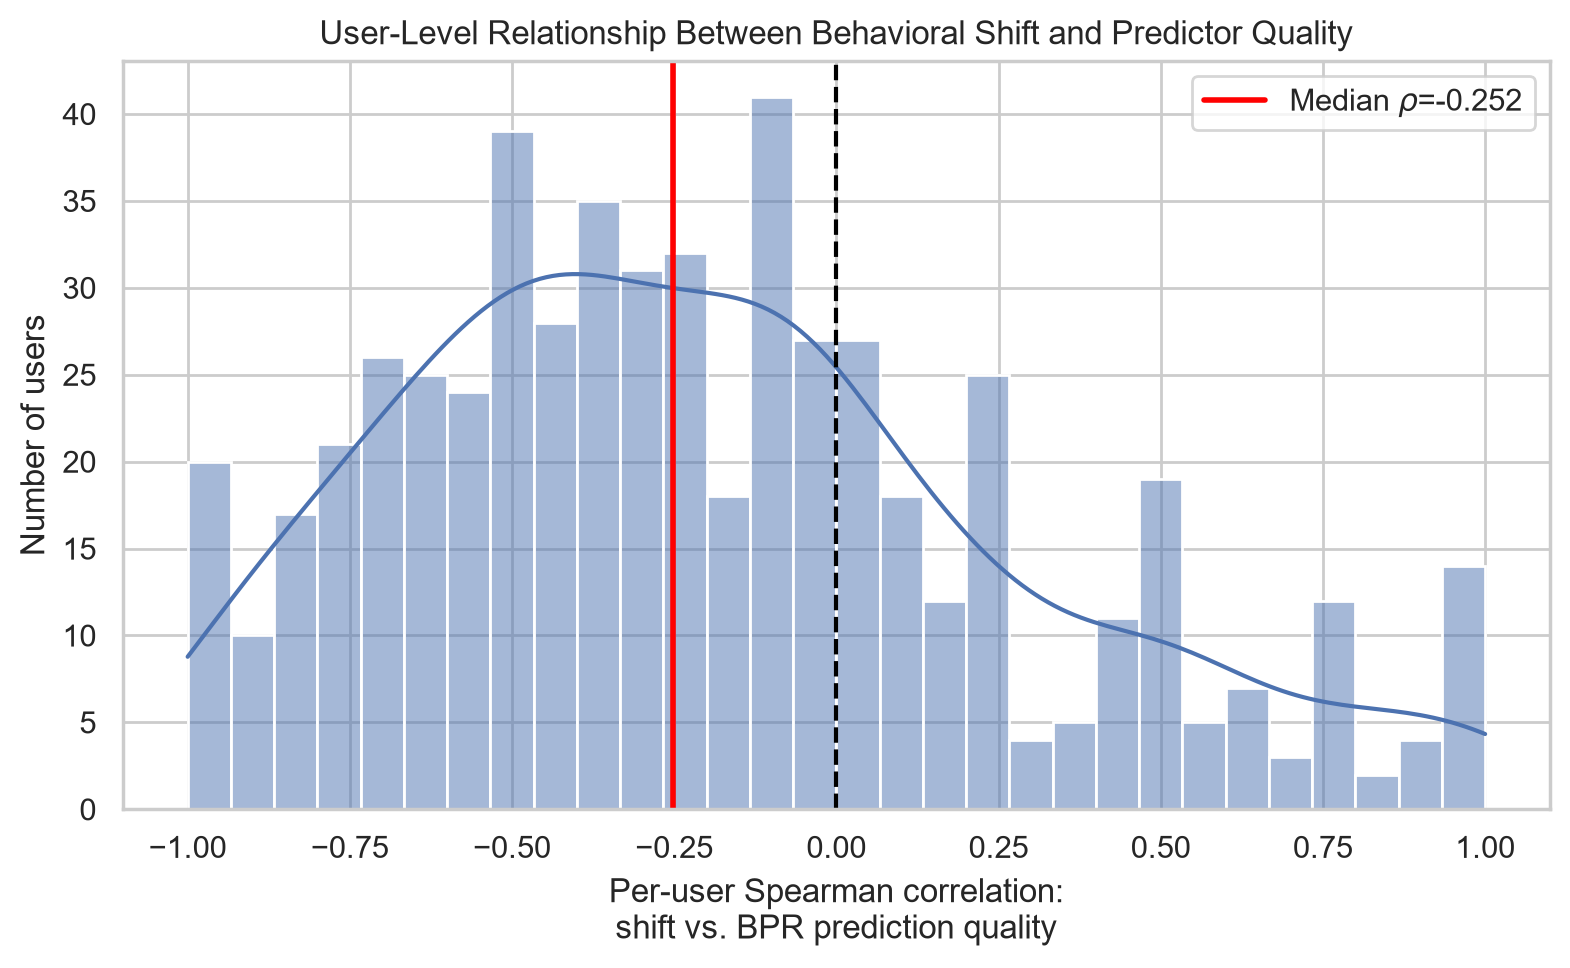
\includegraphics[
        width=0.88\linewidth
    ]{shift_by_user.png}
    \caption{
    Distribution of per-user Spearman correlations between behavioral
    shift and historical BPR prediction quality. The median correlation
    is negative, although substantial user-level heterogeneity remains.
    }
    \label{fig:usercorrelation}
\end{figure}

\subsection{Window-Size Sensitivity}

To determine whether the observed relationship depends strongly on the
choice of 250 interactions per window, the analysis is repeated with
window sizes of 125 and 500.

\begin{table}[H]
\centering
\caption{
Sensitivity of the shift--quality relationship to temporal window
size.
}
\label{tab:sensitivity}
\begin{tabular}{rrrrr}
\toprule
Window
& Users
& Windows
& Overall $\rho$
& Median user $\rho$ \\
\midrule
125 & 736 & 14,153 & -0.383 & -0.284 \\
250 & 595 & 6,642  & -0.359 & -0.252 \\
500 & 405 & 2,848  & -0.334 & -0.300 \\
\bottomrule
\end{tabular}
\end{table}

The fraction of users with negative within-user correlation is 74.0\%,
70.1\%, and 66.1\% for window sizes 125, 250, and 500 respectively.
Thus, while quantitative values vary, the qualitative relationship is
stable across all three temporal resolutions.

% ============================================================
% 6. ROBUST PREDICTION COMBINATION
% ============================================================

\section{Robust Prediction Combination}

\subsection{Sequential Experts}

The robust-learning experiment treats prediction as a combination of
two experts.

The \emph{historical expert} is a frozen BPR model trained before the
evaluation stream.

The \emph{online expert} maintains exponentially decayed recent
interaction counts:
%
\begin{equation}
    c_{u,t}(i)
    =
    \lambda
    c_{u,t-1}(i)
    +
    n_{u,t}(i),
\end{equation}
%
where $\lambda=0.8$ and $n_{u,t}(i)$ denotes interactions with artist
$i$ in the current window. A global-popularity prior is used before
sufficient online observations have accumulated.

Critically, predictions for window $t$ are produced before that
window's observations are incorporated into the online model.

\subsection{Loss}

For expert $e$,
%
\begin{equation}
    \ell_{e,t}
    =
    1
    -
    \operatorname{EventMass@20}_{e,t}.
\end{equation}
%
Thus,
%
\begin{equation}
    0 \leq \ell_{e,t} \leq 1.
\end{equation}

For mixture weight $\alpha_t$ on the historical expert, the expected
mixture loss is
%
\begin{equation}
    \ell_t
    =
    \alpha_t
    \ell_{H,t}
    +
    (1-\alpha_t)
    \ell_{O,t}.
\end{equation}

This quantity corresponds to the expected loss of probabilistically
selecting the historical expert with probability $\alpha_t$ and the
online expert otherwise.

\subsection{Methods}

Five strategies are compared.

\paragraph{Prediction Only.}
%
\begin{equation}
    \alpha_t = 1.
\end{equation}

\paragraph{Online Only.}
%
\begin{equation}
    \alpha_t = 0.
\end{equation}

\paragraph{Static Mixture.}
%
\begin{equation}
    \alpha_t = \alpha,
\end{equation}
%
where $\alpha$ is selected using validation data.

\paragraph{Hedge.}
The historical and online predictors are treated as experts and updated
using exponentially weighted losses
\citep{freund1997decision}.

\paragraph{Shift-Aware Adaptive Trust.}
The proposed candidate mechanism combines behavioral shift and recent
relative expert performance. Let
%
\begin{equation}
    d_t
    =
    (1-\beta)d_{t-1}
    +
    \beta
    \left(
        \ell_{H,t}
        -
        \ell_{O,t}
    \right)
\end{equation}
%
be an exponentially smoothed historical disadvantage.

Before the current window is observed, historical trust is
%
\begin{equation}
    \alpha_t
    =
    \sigma
    \left(
        \operatorname{logit}(\alpha_0)
        -
        \gamma_s s_t
        -
        \gamma_d d_{t-1}
    \right),
\end{equation}
%
where $\sigma$ is the logistic function, $s_t$ is the current
behavioral-shift signal computed from previously observed data,
$\alpha_0$ is baseline trust, and $\gamma_s,\gamma_d$ control
sensitivity to shift and recent relative loss.

All adaptive parameters are selected on the validation stream before
final test evaluation.

% ============================================================
% 7. ROBUST LEARNING RESULTS
% ============================================================

\section{Robust Learning Results}

The final historical models are fitted using training and validation
data. Robust-learning parameters are frozen before the held-out test
stream is evaluated.

The selected validation parameters include a static historical weight
of $0.25$, Hedge learning rate $\eta=2.0$, and shift-aware parameters
%
\[
\alpha_0=0.75,
\qquad
\gamma_s=2.0,
\qquad
\gamma_d=2.0,
\qquad
\beta=0.25.
\]

A total of 736 users satisfy the requirement of at least three complete
250-interaction test windows.

Table~\ref{tab:robustresults} reports final performance.

\begin{table}[H]
\centering
\caption{
Held-out sequential robust-learning results. Lower loss and regret are
better; higher expected EventMass@20 is better.
}
\label{tab:robustresults}
\begin{tabular}{lrrr}
\toprule
Method
& Mean loss
& Expected EventMass@20
& Mean regret \\
\midrule
Online Only
& \textbf{0.6421}
& \textbf{0.3579}
& \textbf{0.0004} \\
Hedge
& 0.6815
& 0.3185
& 0.4179 \\
Static Mixture
& 0.7158
& 0.2842
& 1.5119 \\
Shift-Aware Trust
& 0.7599
& 0.2401
& 2.2557 \\
Prediction Only
& 0.9369
& 0.0631
& 6.0464 \\
\bottomrule
\end{tabular}
\end{table}

Figure~\ref{fig:robustcomparison} visualizes expected EventMass@20.

\begin{figure}[H]
    \centering
    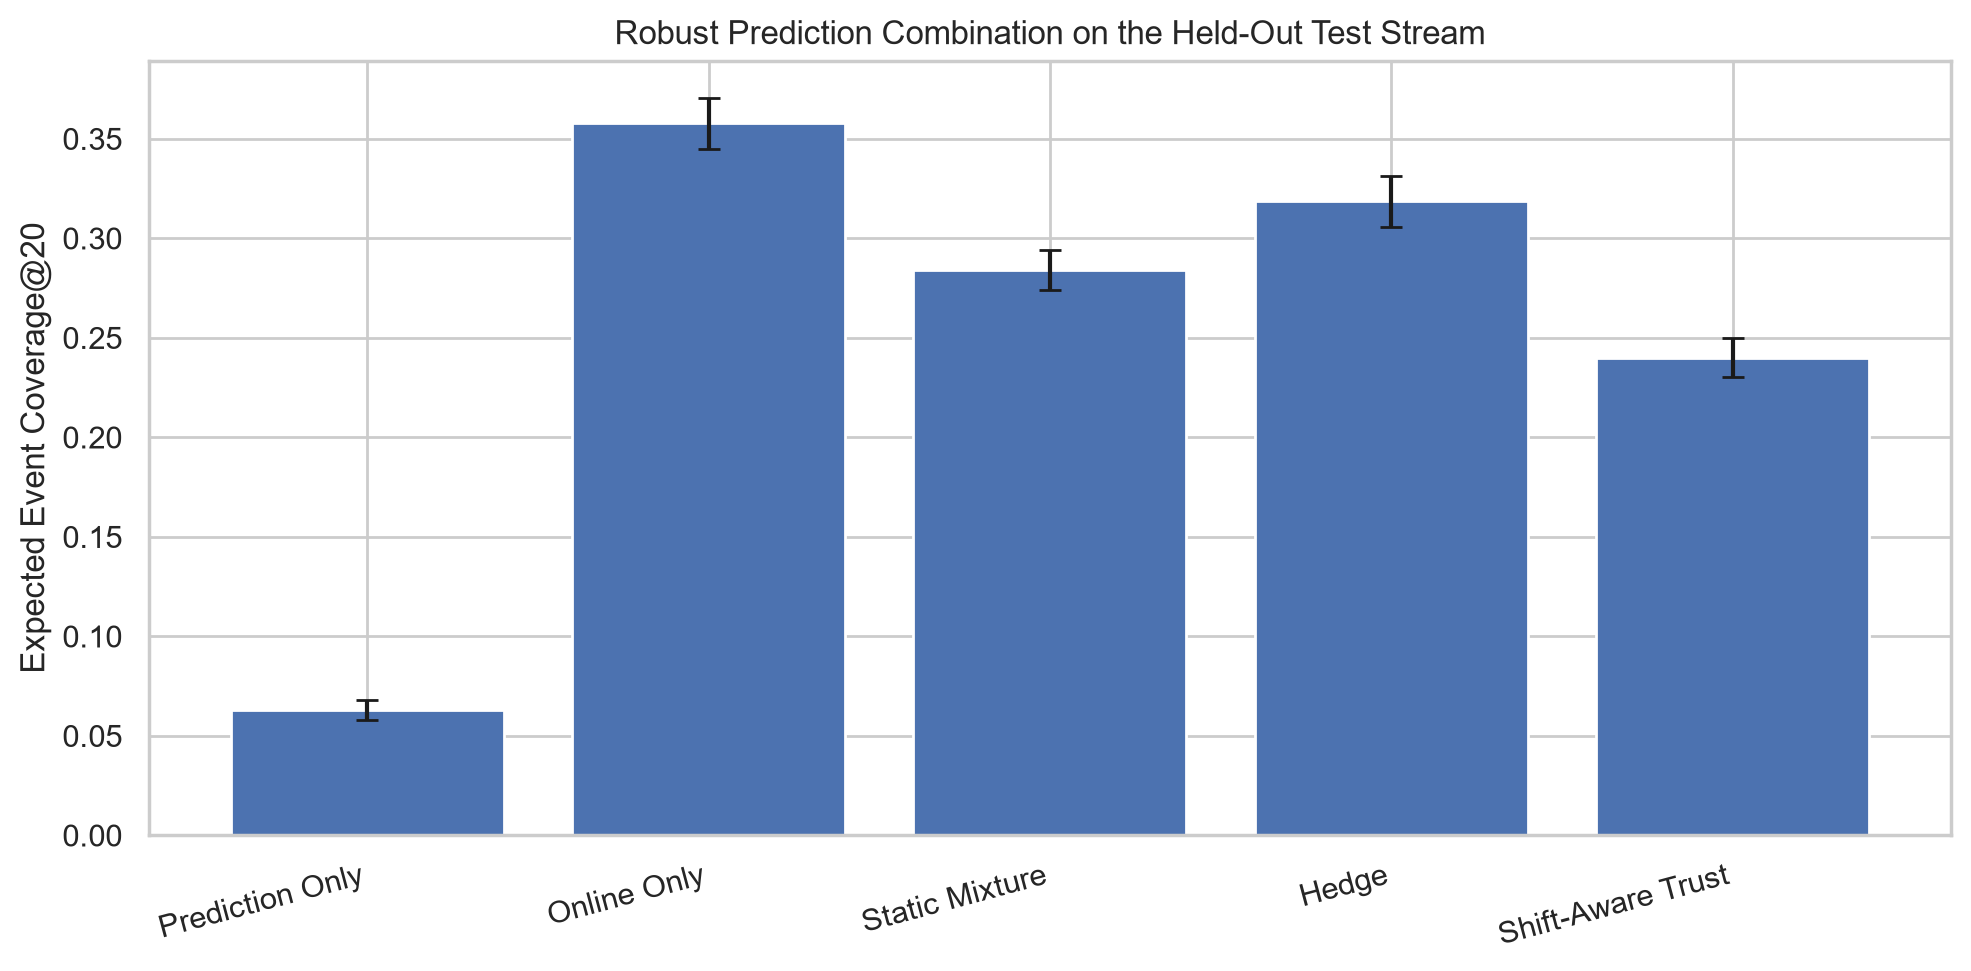
\includegraphics[
        width=0.88\linewidth
    ]{robust_learning_comparison.png}
    \caption{
    Final robust-learning comparison on the held-out sequential test
    stream. Error bars show 95\% normal-approximation intervals over
    user-level mean losses.
    }
    \label{fig:robustcomparison}
\end{figure}

\subsection{Historical Prediction Becomes Weak}

Prediction Only performs substantially worse than every strategy that
incorporates online evidence. Its expected EventMass@20 is only 0.0631.

This result is consistent with the shift analysis: historical
personalization can become severely stale when future behavior differs
from the historical distribution.

\subsection{Online Adaptation Dominates}

Online Only achieves the strongest average performance with expected
EventMass@20 of 0.3579 and near-zero mean regret relative to the better
fixed expert.

This implies that, under the current experimental design, the recent
interaction stream contains substantially more useful information than
the frozen historical BPR predictor.

Hedge provides the strongest combined-expert strategy, obtaining
EventMass@20 of 0.3185. Its multiplicative update rapidly decreases the
weight assigned to BPR once the online expert demonstrates lower loss.

\subsection{Why Shift-Aware Trust Underperforms}

The proposed shift-aware method improves substantially over Prediction
Only but does not outperform Static Mixture, Hedge, or Online Only.

Figure~\ref{fig:trust} provides a mechanistic explanation.

\begin{figure}[H]
    \centering
    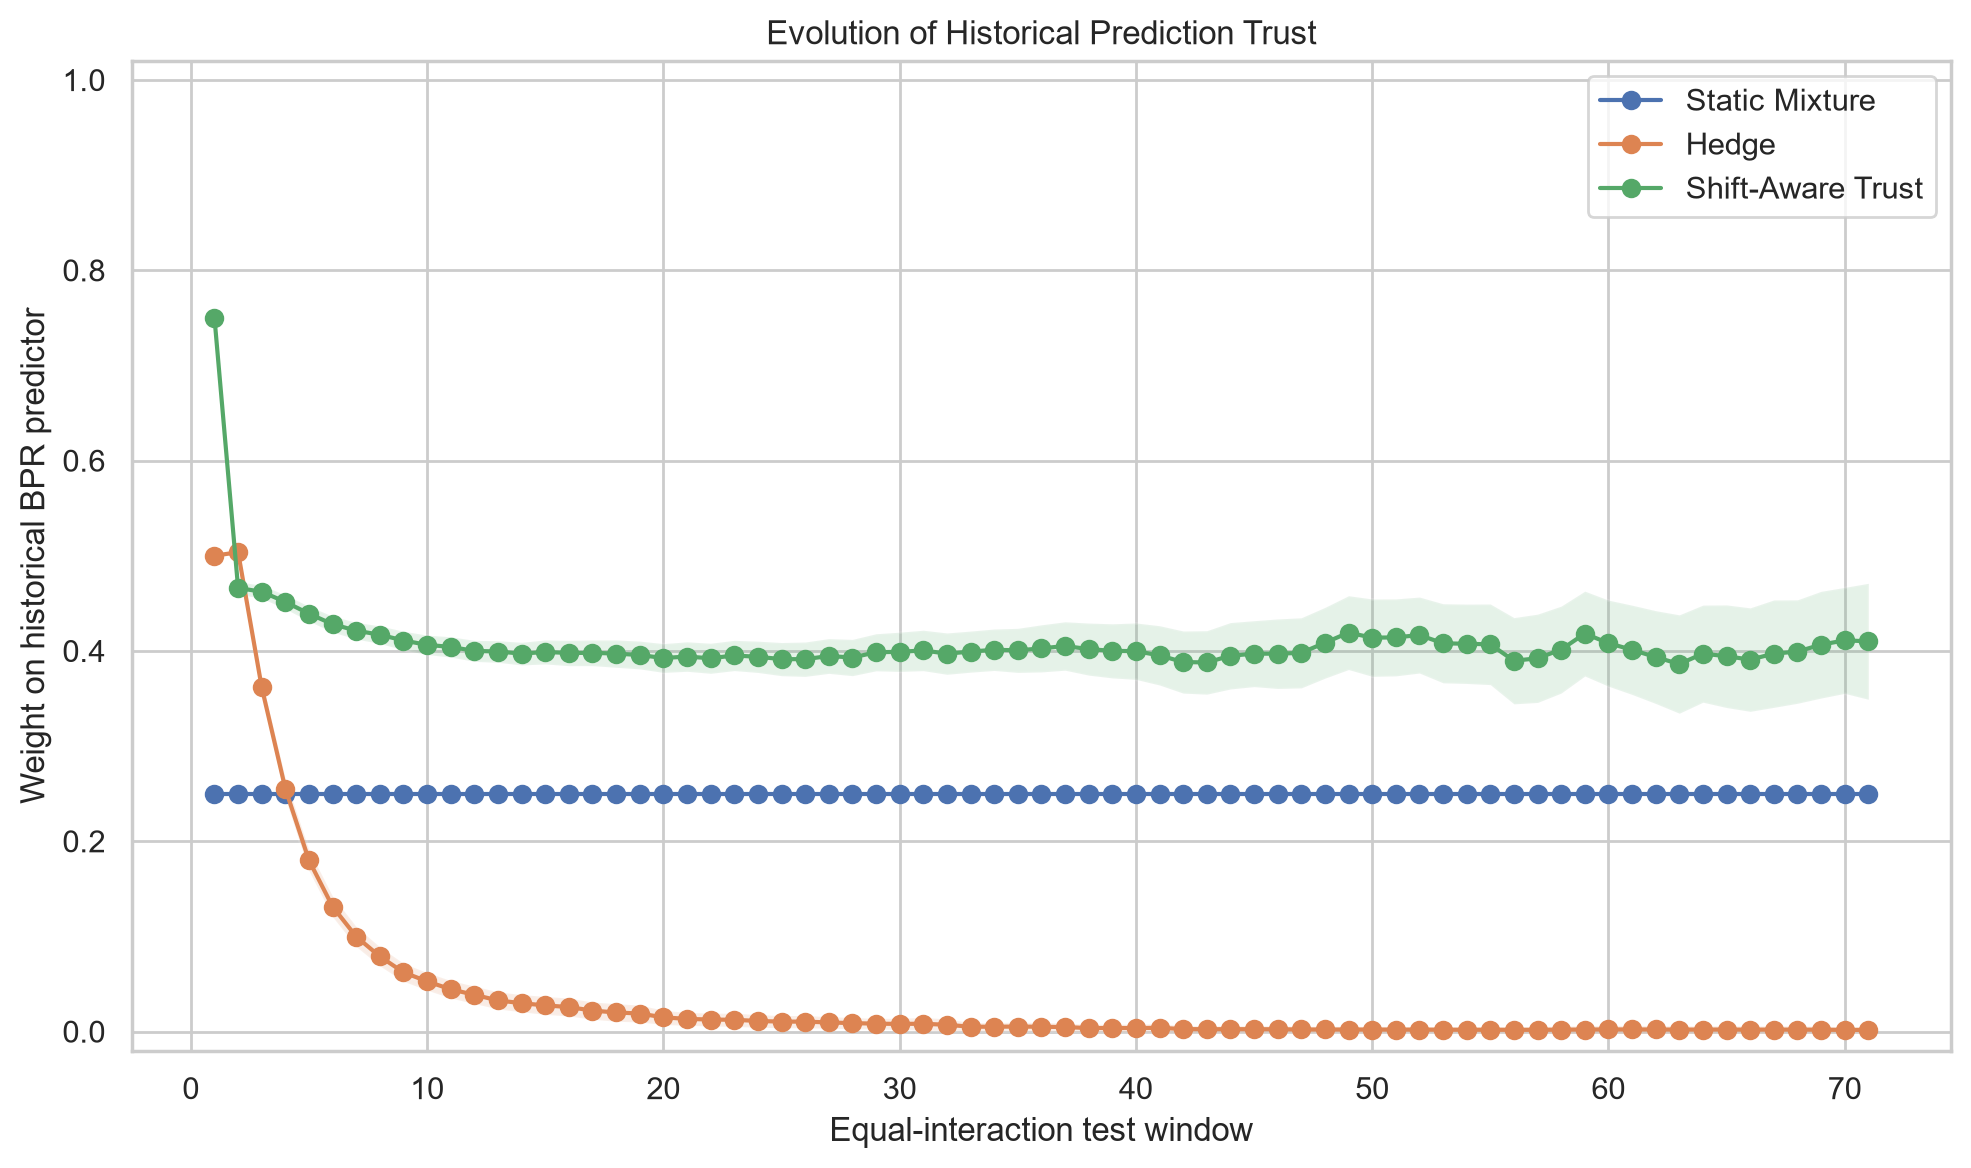
\includegraphics[
        width=0.88\linewidth
    ]{trust_over_time.png}
    \caption{
    Mean weight placed on the frozen historical BPR predictor across
    sequential test windows. Hedge rapidly reduces historical trust
    toward zero, whereas the selected shift-aware rule stabilizes around
    a considerably larger historical weight.
    }
    \label{fig:trust}
\end{figure}

The selected shift-aware method retains approximately 0.4 historical
weight over much of the stream. Hedge, by contrast, rapidly learns to
place almost no weight on BPR.

The negative result therefore does not imply that the behavioral shift
signal contains no information. Milestone 3 demonstrates that shift is
associated with predictor degradation. Instead, the result shows that
the current mapping
%
\[
s_t
\longrightarrow
\alpha_t
\]
%
does not withdraw historical trust aggressively enough relative to the
strength of the online expert.

Figure~\ref{fig:shiftrobust} further shows performance as behavioral
shift increases.

\begin{figure}[H]
    \centering
    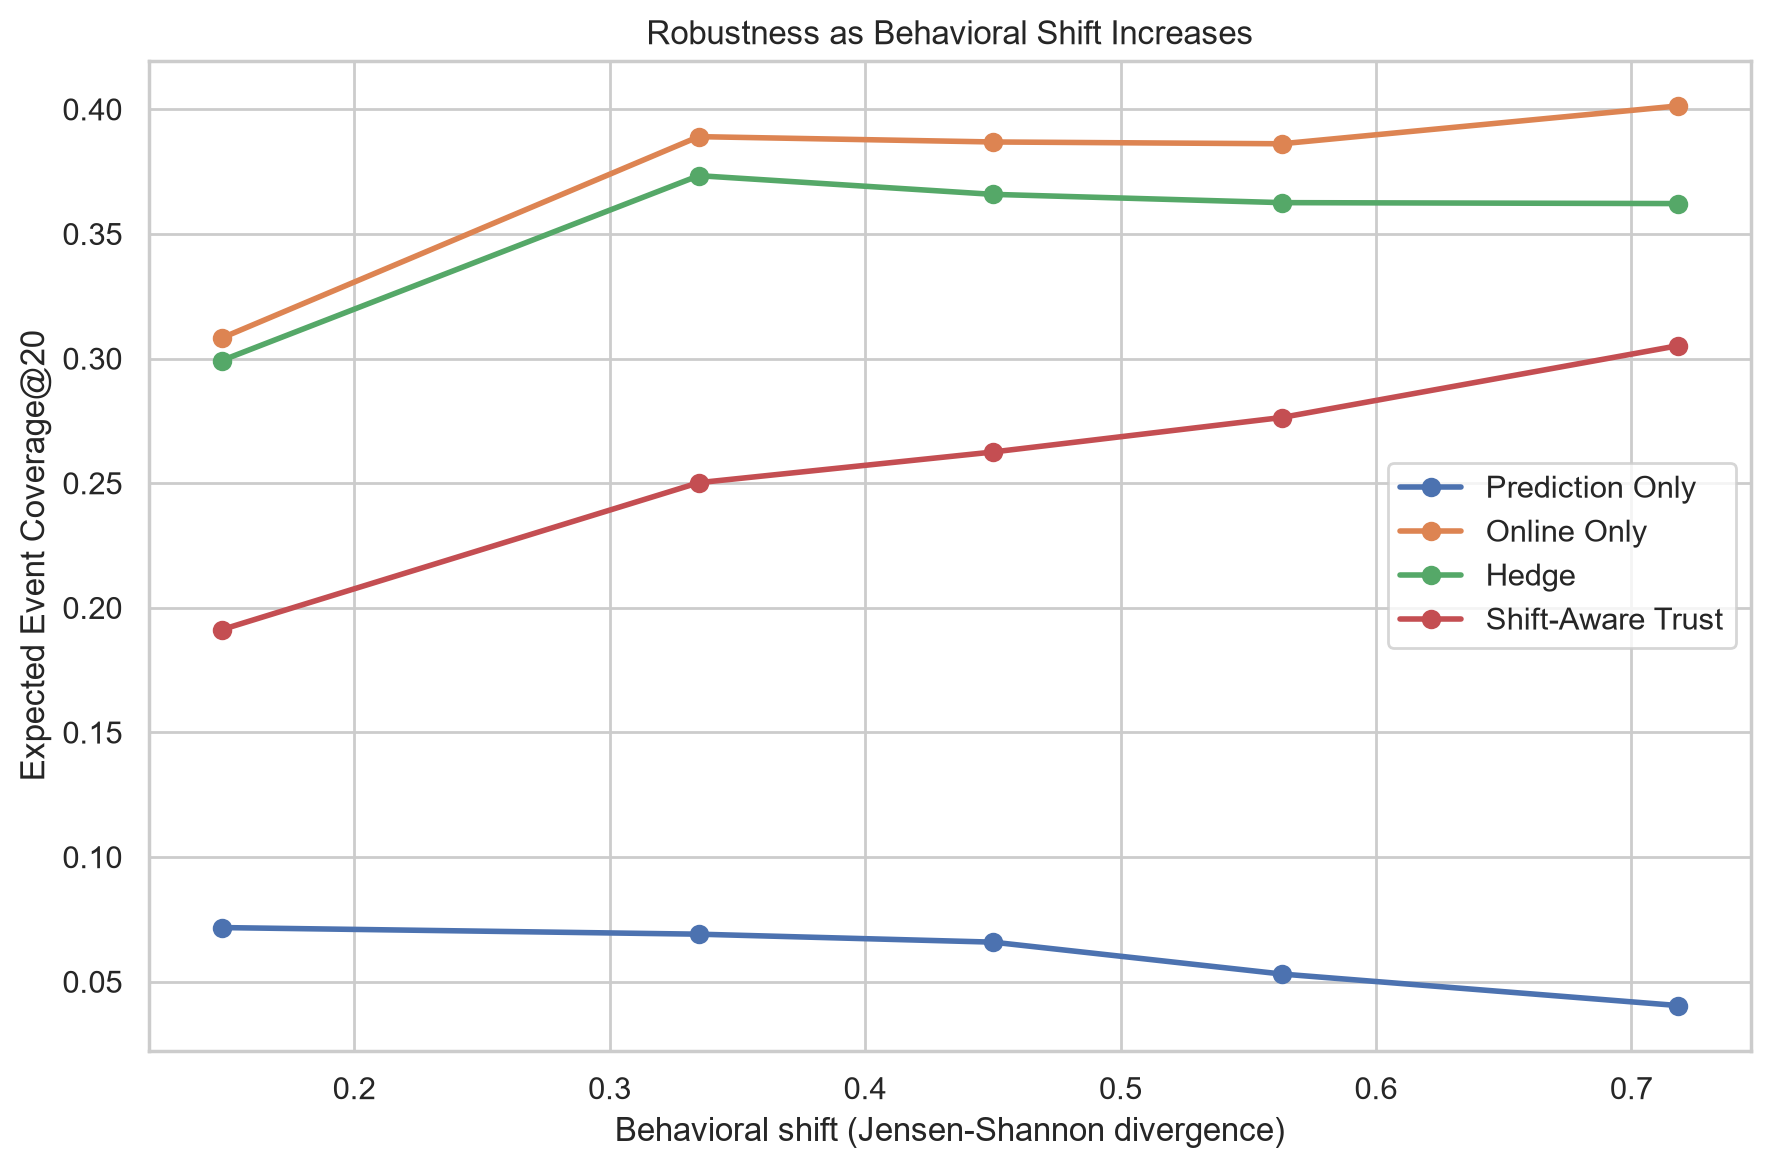
\includegraphics[
        width=0.88\linewidth
    ]{performance_by_shift.png}
    \caption{
    Expected EventMass@20 across behavioral-shift quintiles. The
    historical predictor deteriorates as shift increases. Online
    adaptation remains strongest across the observed shift range, while
    Hedge provides the strongest mixed-expert strategy.
    }
    \label{fig:shiftrobust}
\end{figure}

% ============================================================
% 8. DISCUSSION
% ============================================================

\section{Discussion}

The experiments support three principal conclusions.

First, temporal behavioral shift is measurable and associated with
historical-model degradation. This relationship appears both in pooled
analysis and, importantly, within individual users. Its qualitative
stability across several window sizes suggests that it is not merely an
artifact of one arbitrary temporal resolution.

Second, detecting shift and responding optimally to shift are different
problems. Jensen--Shannon divergence contains information about
historical-predictor reliability, yet the explicit shift-aware gating
rule does not outperform loss-adaptive Hedge.

Third, the strong Online Only result demonstrates that historical
predictions need not always be beneficial. The algorithms-with-
predictions perspective often seeks a balance between exploiting
accurate advice and remaining robust when advice fails. In this
particular dataset and evaluation stream, the learned advice becomes
weak enough that rapid adaptation is generally preferable.

This negative result is useful for future algorithm design. A more
competitive shift-aware method may require a mechanism capable of
distinguishing between:

\begin{itemize}
    \item transient behavioral variation;
    \item persistent distribution shift;
    \item regions in which historical predictions remain useful; and
    \item cases where the online predictor has accumulated sufficient
    evidence to supersede historical information.
\end{itemize}

A single global logistic mapping from divergence to trust may be too
restrictive.

% ============================================================
% 9. LIMITATIONS
% ============================================================

\section{Limitations}

Several limitations constrain the conclusions.

\paragraph{Single dataset.}
The study evaluates one historical music-consumption dataset. Results
should not be interpreted as universal properties of modern
recommender systems.

\paragraph{Historical data collection.}
The Last.fm observations are not representative of current music
consumption. The experiments study algorithmic behavior under temporal
shift rather than contemporary popularity.

\paragraph{Active-user selection.}
Equal-interaction windows require sufficiently active users. At the
primary setting, only 595 validation users and 736 test users satisfy
the minimum-window criterion. Conclusions therefore emphasize active
listeners.

\paragraph{Artist-level identifiers.}
Normalized artist names are used as operational item identifiers.
Name collisions or spelling inconsistencies may introduce noise.

\paragraph{Observational shift analysis.}
The negative association between Jensen--Shannon divergence and
historical-predictor quality does not establish a causal relationship.

\paragraph{Simple online expert.}
The online model uses exponentially decayed interaction counts rather
than a sophisticated sequential neural recommender. This simplicity is
intentional for isolating the expert-combination problem, but limits
the scope of conclusions about recommendation architectures.

\paragraph{Mixture interpretation.}
Combined strategies are evaluated by expected convex mixture loss.
This corresponds to randomized expert selection rather than explicitly
constructing a new deterministic top-$K$ ranking from heterogeneous
score spaces.

\paragraph{Initial shift-aware formulation.}
The proposed trust mechanism constitutes an initial candidate rather
than a theoretically optimal algorithm. Its underperformance should be
interpreted as evidence about the formulation, not as evidence that
distribution-shift signals cannot be useful.

% ============================================================
% 10. CONCLUSION
% ============================================================

\section{Conclusion}

This study investigated robust use of historical machine-learning
predictions under temporal behavioral shift.

Using approximately 18.5 million processed Last.fm interactions, we
found a consistent negative association between divergence from
historical listening behavior and the quality of a frozen BPR
predictor. The result persisted across several equal-interaction window
sizes and was observable within a majority of individual users.

We then formulated sequential recommendation as an online
expert-combination problem. Exclusive reliance on historical prediction
performed poorly, while online adaptation achieved the strongest
held-out performance. Hedge successfully learned to discount the stale
historical predictor and was the strongest mixed-expert strategy.

A shift-aware adaptive trust rule improved substantially over
Prediction Only but did not outperform Hedge or Online Only. Inspection
of its learned trust trajectory showed that it retained excessive
historical weight after the online expert had become substantially more
reliable.

The central conclusion is therefore twofold: behavioral distribution
shift provides useful evidence about predictor reliability, but
effective robustness requires more than detecting that shift. Future
work should investigate theoretically grounded mechanisms that convert
local distribution-shift evidence into prediction trust while retaining
the worst-case robustness properties of online expert algorithms.

% ============================================================
% REPRODUCIBILITY
% ============================================================

\section*{Reproducibility Statement}

The complete preprocessing pipeline, recommendation baselines,
distribution-shift analysis, robust-learning algorithms, unit tests,
figures, and experiment scripts are maintained in the accompanying
research repository.

All major experiments use fixed random seeds. Hyperparameters for BPR
and robust expert-combination methods are selected using validation
data. Final robust-learning comparisons use the held-out chronological
test stream.

The Last.fm source data are not redistributed in the repository and
must be obtained separately under the dataset's applicable
non-commercial-use conditions.

% ============================================================
% BIBLIOGRAPHY
% ============================================================

\bibliographystyle{plainnat}
\bibliography{references}

\end{document}
